% This text is proprietary.
% It's a part of presentation made by myself.
% It may not used commercial.
% The noncommercial use such as private and study is free
% Sep. 2005 
% Author: Sascha Frank 
% University Freiburg 
% www.informatik.uni-freiburg.de/~frank/
% additional use of \usepackage{beamerthemesplit}
\documentclass{beamer}
\usepackage{beamerthemesplit} % new 
\usepackage[utf8]{inputenc}
\begin{document}
\title{Technologies mobiles} 
\author{Olivier Levitt} 
\date{\today} 

\frame{
\titlepage

\includegraphics[width=60pt]{google-android.jpg}
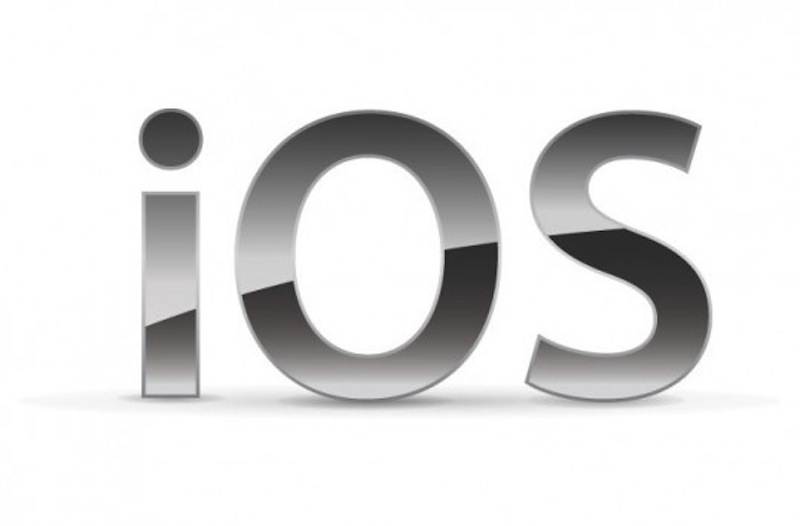
\includegraphics[width=60pt]{ios.png}
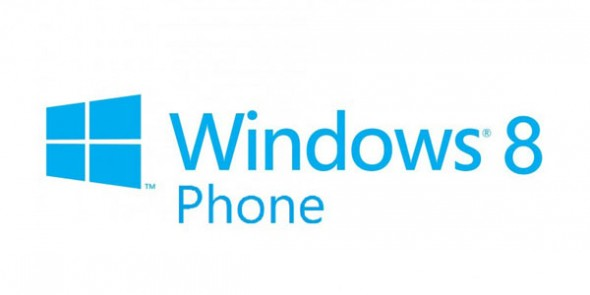
\includegraphics[width=60pt]{wp8.jpg}

\includegraphics[width=60pt]{bb10.jpg}
} 

\frame{\frametitle{Sommaire}\tableofcontents} 

\section{Introduction} 
\subsection{De quoi on va parler ?}
\subsection{Comparaison des différents OS mobile}

\section{Les spécificités du développement mobile} 
\subsection{Spécificités techniques}

\section{Le développement sur android} 
\subsection{Mise en place}
\subsection{Hello world}
\subsection{Les composants}



\frame{ 
Without title somethink is missing. 
}


\end{document}
